\section{Příručka k použití}
Pro spuštění programu je třeba mít nainstalované tyto programy:
\begin{itemize}
	\item .NET Core SDK verze 3.1
	\item Node.js verze 12 nebo 14
	\item lokální instance Microsoft SQL Server databáze
	\item nástroj CLI tools for Entity Framework Core
	\item aplikace Postman, nástroj curl, nebo jiný program, který umožňuje posílat HTTP POST dotazy
\end{itemize}

V kořenovém adresáři aplikace zadáme do příkazové řádky nejprve následující příkaz.

\begin{lstlisting}
dotnet ef database update --project CourseManagementSystem.Data --startup-project CourseManagementSystem.API
\end{lstlisting}

Dojde k vytvoření databáze na lokální instanci SQL Serveru.
Pro spuštění aplikace zadáme tyto příkazy:
\begin{lstlisting}
dotnet build
cd CourseManagementSystem.API
dotnet run
\end{lstlisting}

Tímto dojde ke spuštění aplikace. Ve výpisu příkazu \textit{dotnet run} na příkazové řádce bychom nyní měli vidět URL, na které se aplikace nachází (typicky je to URL \url{https://localhost:5001}). Otevřeme webový prohlížeč na této URL a následně se zobrazí domovská stránka aplikace.

\subsection{Generování testovacích dat}

\begin{itemize}
	\item Nejprve ve webovém rozhraní aplikace manuálně provedeme registraci čtyř uživatelů podle postupu v uživatelské dokumentaci \ref{UserDoc} (můžeme například použít heslo \textit{Password01.}).

	\item Otevřeme databázi s názvem \textit{CMS} na lokální instanci SQL Serveru a provedeme následujicí SQL dotaz.
	\begin{lstlisting}
	select u.Id, u.UserName from AspNetUsers u
	\end{lstlisting}
	
	Dostaneme seznam všech registrovaných uživatelů s jejich identifikátory, příklad výsledku dotazu můžeme vidět níže.
	
	\begin{lstlisting}
	Id										UserName
	f9865b52-175d-45cc-9116-4737d8f00e5e	a@gmail.com
	4e7a88fb-dcab-46c4-85d5-aebadbd64bb0	b@gmail.com
	93ed1d4d-4020-44a0-b06d-fb182f1c6243	c@gmail.com
	48073c12-29e5-4200-81e5-a9ce2ef0980b	d@gmail.com
	\end{lstlisting}
	
	\item Provedeme HTTP POST dotaz s prázdným tělem na URL
	
	\url{https://localhost:5001/api/testData/generate/{person1Id}/{person2Id}/{person3Id}/{person4Id}}
	
	Do proměnných \textit{\{person1Id\}}, apod. dosadíme identifikátory jednotlivých osob. V našem příkladu tedy například místo \textit{\{person1Id\}} dosadíme řetězec \textit{f9865b52-175d-45cc-9116-4737d8f00e5e}.
	
	HTTP POST dotaz můžeme provést například pomocí aplikaci Postman nebo využitím nástroje curl.
	
	\begin{itemize}
		\item V případě, že používáme aplikaci Postman, pošleme požadavek podobně jako na příkladu \ref{fig:Postman}.
		\item Pokud používáme nástroj curl, tak provedeme v příkazové řádce příkaz uvedený v kódu \ref{curl}. Do příslušných částí URL vložíme identifikátory osob.
	\end{itemize}

	\item Tento HTTP dotaz zavolá metodu \textit{GenerateTestData} v Controlleru \textit{TestDataController}, která vygeneruje testovací data, jenž se uloží do databáze. 
	
	\item Aplikace nyní obsahuje testovací data. Podle návodu uvedeného v uživatelské dokumentaci \ref{UserDoc} se přihlásíme jako jeden z uživatelů.
\end{itemize}

\begin{figure}
	\centering
	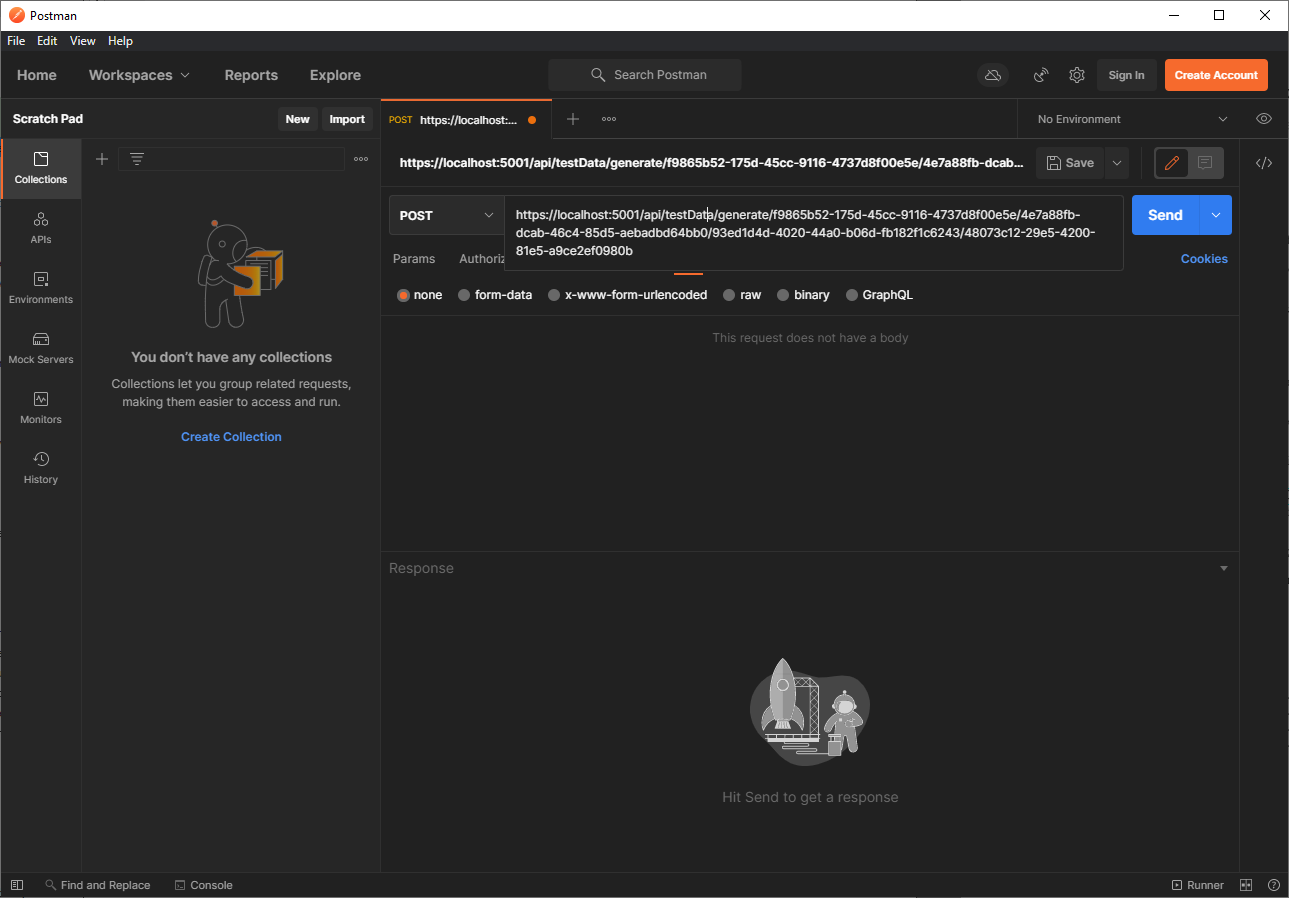
\includegraphics[width=\textwidth]{postman.PNG}
	\caption{Příklad odeslání HTTP POST požadavku v aplikaci Postman}
	\label{fig:Postman}
\end{figure}

\begin{program}
	\begin{lstlisting}
		curl -d {} https://localhost:5001/api/testData/generate/
		{person1Id}/{person2Id}/{person3Id}/{person4Id}
	\end{lstlisting}
	\caption{Odeslání HTTP POST požadavku pomocí programu curl}
	\label{curl}
\end{program}